\chapter{Parent Portal (mobile app)}

After signing in, a parent sees five buttons at the bottom of the
screen:

\begin{center}
\textbf{Attendance} \quad \textbf{Schedule} \quad \textbf{Activity}
\quad \textbf{Feedback} \quad \textbf{Alerts}
\end{center}

If you have more than one child in the school, a small selector at the
top of the screen lets you switch between children -- everything on the
screen then shows that child's information.

% ----------------------------------------------------------------------
\section{Attendance -- was my child at school?}

The \textbf{Attendance} tab has two views, switchable at the top:

\subsection{Daily view}
One line per day: a green tick if the child was present, the
\textbf{arrival time} at the gate and the \textbf{departure time}.

\subsection{Movements view}
The full trail of the day, recorded automatically by the room antennas:
entered Room 101 at 08:02, left at 08:59, entered the Library at 10:15,
and so on. Nothing needs to be typed by anyone -- walking through a door
is enough.

\begin{figure}[H]
\centering
\begin{tikzpicture}[font=\sffamily]
  \phoneframe{Hi, Mr. Khan}
  \node[anchor=west, text=black!70] at (0.35,8.60) {\scriptsize Ali Khan \textbullet{}  Grade 7 A \textbullet{}  G7-001};
  \draw[rounded corners=6pt, fill=white, draw=campusblue] (0.9,7.6) rectangle (4.3,8.25);
  \node[text=campusblue] at (1.75,7.92) {\scriptsize\textbf{Daily}};
  \node[text=black!45] at (3.45,7.92) {\scriptsize Movements};
  \appcard{6.3}{\checkmark}{Mon, 17 Aug}{In: 07:58 am \; Out: 01:32 pm}
  \appcard{5.1}{\checkmark}{Tue, 18 Aug}{In: 08:03 am \; Out: 01:30 pm}
  \appcard{3.9}{$\times$}{Wed, 19 Aug}{Absent}
  \appcard{2.7}{\checkmark}{Thu, 20 Aug}{In: 07:55 am \; Out: 01:31 pm}
  \navbar
  \navitem{0.70}{Attendance}{campusblue}
  \navitem{1.70}{Schedule}{black!55}
  \navitem{2.60}{Activity}{black!55}
  \navitem{3.50}{Feedback}{black!55}
  \navitem{4.40}{Alerts}{black!55}
\end{tikzpicture}
\hspace{0.8cm}
\begin{tikzpicture}[font=\sffamily]
  \phoneframe{Hi, Mr. Khan}
  \node[anchor=west, text=black!70] at (0.35,8.60) {\scriptsize Ali Khan \textbullet{}  Grade 7 A \textbullet{}  G7-001};
  \draw[rounded corners=6pt, fill=white, draw=campusblue] (0.9,7.6) rectangle (4.3,8.25);
  \node[text=black!45] at (1.75,7.92) {\scriptsize Daily};
  \node[text=campusblue] at (3.45,7.92) {\scriptsize\textbf{Movements}};
  \appcard{6.3}{$\rightarrow$}{Entered Main Gate}{Gate \textbullet{}  07:58 am}
  \appcard{5.1}{$\rightarrow$}{Entered Room 101}{Classroom \textbullet{}  08:02 am}
  \appcard{3.9}{$\leftarrow$}{Left Room 101}{Classroom \textbullet{}  08:59 am}
  \appcard{2.7}{$\rightarrow$}{Entered Library}{Library \textbullet{}  10:15 am}
  \navbar
  \navitem{0.70}{Attendance}{campusblue}
  \navitem{1.70}{Schedule}{black!55}
  \navitem{2.60}{Activity}{black!55}
  \navitem{3.50}{Feedback}{black!55}
  \navitem{4.40}{Alerts}{black!55}
\end{tikzpicture}
\caption{Attendance tab: the Daily view (left) and the room-by-room
Movements view (right). Illustrations of the app screens.}
\end{figure}

\tipbox{Pull the list downwards with your finger to refresh it.}

% ----------------------------------------------------------------------
\section{Schedule -- the full semester timetable}

Tap \textbf{Schedule} to see your child's timetable for the whole
semester, day by day: subject, time, teacher and room. Whenever the
school updates the timetable, the app always shows the latest version --
no paper needed.

\begin{figure}[H]
\centering
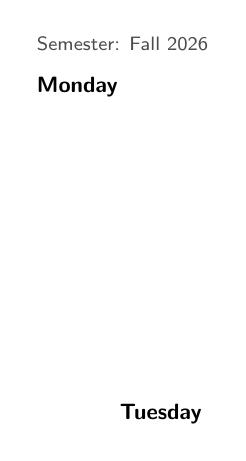
\begin{tikzpicture}[font=\sffamily]
  \phoneframe{Hi, Mr. Khan}
  \node[anchor=west, text=black!70] at (0.35,8.60) {\scriptsize Semester: Fall 2026};
  \node[anchor=west] at (0.35,8.05) {\footnotesize\textbf{Monday}};
  \appcard{6.8}{}{Mathematics}{08:00--09:00 \textbullet{}  Ms. Fatima \textbullet{}  Room 101}
  \appcard{5.6}{}{English}{09:00--10:00 \textbullet{}  Mr. Adeel \textbullet{}  Room 101}
  \appcard{4.4}{}{Physics Lab}{10:15--11:45 \textbullet{}  Ms. Sana \textbullet{}  Physics Lab}
  \node[anchor=west] at (0.35,3.9) {\footnotesize\textbf{Tuesday}};
  \appcard{2.7}{}{Computer Science}{08:00--09:00 \textbullet{}  Mr. Bilal \textbullet{}  Computer Lab}
  \navbar
  \navitem{0.70}{Attendance}{black!55}
  \navitem{1.70}{Schedule}{campusblue}
  \navitem{2.60}{Activity}{black!55}
  \navitem{3.50}{Feedback}{black!55}
  \navitem{4.40}{Alerts}{black!55}
\end{tikzpicture}
\caption{Schedule tab: the whole semester, grouped by day
(illustration).}
\end{figure}

% ----------------------------------------------------------------------
\section{Activity -- what teachers say about my child}

Tap \textbf{Activity} to read every report a teacher has written about
your child: test results, homework status, behaviour notes, sports
achievements. Each report shows the category, the date, the teacher's
name, the remarks and (when given) a grade.

You do not have to keep checking: whenever a teacher writes a new
report, your phone receives a notification immediately.

\begin{figure}[H]
\centering

\begin{tikzpicture}[font=\sffamily]
  \phoneframe{Hi, Mr. Khan}
  \appcard{7.3}{A}{Math quiz}{TestResult \textbullet{}  18 Aug \textbullet{}  Excellent work \textbullet{}  Ms. Fatima}
  \appcard{6.1}{}{Homework complete}{HomeworkStatus \textbullet{}  17 Aug \textbullet{}  Mr. Adeel}
  \appcard{4.9}{}{Football trials selected}{Sports \textbullet{}  15 Aug \textbullet{}  Coach Imran}
  \appcard{3.7}{B+}{English essay}{TestResult \textbullet{}  12 Aug \textbullet{}  Good effort \textbullet{}  Mr. Adeel}
  \navbar
  \navitem{0.70}{Attendance}{black!55}
  \navitem{1.70}{Schedule}{black!55}
  \navitem{2.60}{Activity}{campusblue}
  \navitem{3.50}{Feedback}{black!55}
  \navitem{4.40}{Alerts}{black!55}
\end{tikzpicture}
\caption{Activity tab: all teacher reports in one place
(illustration).}
\end{figure}

% ----------------------------------------------------------------------
\section{Feedback -- talk to the school}

Tap \textbf{Feedback} to send a message to the school in one of the
fixed columns (categories):

\begin{center}
Teaching \; \textbullet{}  \; Homework \; \textbullet{}  \; Facilities \; \textbullet{}  \; Transport \; \textbullet{}  \;
Discipline \; \textbullet{}  \; Suggestion \; \textbullet{}  \; Complaint
\end{center}

\begin{enumerate}[itemsep=2pt]
  \item Choose which child the feedback is about (if you have several).
  \item Choose the category from the list.
  \item Type your message and tap \textbf{Submit}.
\end{enumerate}

Below the form you can see all your earlier messages, their status
(Open / Replied / Closed) and the school's written reply. When the
school replies, you also get a phone notification.

\begin{figure}[H]
\centering
\begin{tikzpicture}[font=\sffamily]
  \phoneframe{Hi, Mr. Khan}
  \node[anchor=west] at (0.35,8.45) {\footnotesize\textbf{Send feedback}};
  \draw[rounded corners=3pt, fill=white, draw=black!25] (0.35,7.6) rectangle (4.85,8.15);
  \node[anchor=west, text=black!60] at (0.55,7.87) {\scriptsize Category: Teaching \; $\blacktriangledown$};
  \draw[rounded corners=3pt, fill=white, draw=black!25] (0.35,6.0) rectangle (4.85,7.4);
  \node[anchor=west, text=black!60] at (0.55,6.95) {\scriptsize Ali says he enjoys the new};
  \node[anchor=west, text=black!60] at (0.55,6.60) {\scriptsize math activities. Thank you!};
  \draw[rounded corners=3pt, fill=campusblue] (0.35,5.2) rectangle (4.85,5.8);
  \node[text=white] at (2.6,5.5) {\scriptsize\textbf{Submit}};
  \node[anchor=west] at (0.35,4.6) {\footnotesize\textbf{Previous feedback}};
  \appcard{3.3}{}{[Transport] Bus is late}{Replied \textbullet{}  School reply: New route from Monday}
  \navbar
  \navitem{0.70}{Attendance}{black!55}
  \navitem{1.70}{Schedule}{black!55}
  \navitem{2.60}{Activity}{black!55}
  \navitem{3.50}{Feedback}{campusblue}
  \navitem{4.40}{Alerts}{black!55}
\end{tikzpicture}
\caption{Feedback tab: fixed categories, your message, and the school's
replies below (illustration).}
\end{figure}

% ----------------------------------------------------------------------
\section{Alerts -- every notification in one list}

Tap \textbf{Alerts} to see everything the school has sent you:

\begin{itemize}[itemsep=2pt]
  \item \textbf{Gate alerts} -- ``Ali Khan entered school at 07:58''
        the moment it happens;
  \item \textbf{Daily summary} -- every evening: arrival, departure,
        rooms attended, teacher updates of the day;
  \item \textbf{Weekly summary} -- every Friday, the whole week at a
        glance;
  \item \textbf{Activity alerts} -- a teacher wrote a new report;
  \item \textbf{Feedback replies} -- the school answered your message.
\end{itemize}

Unread notifications are shown in bold; tap one to mark it as read.

\begin{figure}[H]
\centering

\begin{tikzpicture}[font=\sffamily]
  \phoneframe{Hi, Mr. Khan}
  \appcard{7.3}{}{Ali Khan entered school}{GateEntry \textbullet{}  07:58 am}
  \appcard{6.1}{}{New TestResult update for Ali Khan}{Activity \textbullet{}  Math quiz -- A}
  \appcard{4.9}{}{Daily report -- Ali Khan -- 17 Aug}{Arrived 07:58, departed 01:32, 4 rooms}
  \appcard{3.7}{}{Weekly report -- week ending 14 Aug}{Present 5 of 5 days}
  \navbar
  \navitem{0.70}{Attendance}{black!55}
  \navitem{1.70}{Schedule}{black!55}
  \navitem{2.60}{Activity}{black!55}
  \navitem{3.50}{Feedback}{black!55}
  \navitem{4.40}{Alerts}{campusblue}
\end{tikzpicture}
\caption{Alerts tab: gate events, daily and weekly summaries, teacher
updates and replies (illustration).}
\end{figure}
